\setcounter{mtc}{4} %indique le numéro réel du chapitre, pour la mini table des matières
\setcounter{chapter}{0}
\chapter{Project Context and Scope}
\minitoc  %insert la minitoc

\graphicspath{{Chapitre1/figures/}}
%==============================================================================
\pagestyle{fancy}
\fancyhf{}
\fancyhead[R]{\bfseries\chaptername~\thechapter. }
\fancyfoot[R]{\thepage}
\renewcommand{\headrulewidth}{0.5pt}
\renewcommand{\footrulewidth}{0pt}
%\renewcommand{\chaptermark}[1]{\markright{\MakeUppercase{\chaptername~\thechapter. #1 }}{}}
%\renewcommand{\sectionmark}[1]{\markright{\thechapter.\thesection~ #1}}

\begin{spacing}{1.2}
    %==============================================================================

    \section*{Introduction}
    In this first chapter we will present the Paul Scherrer Institute, the host company of the project.
    We will also introduce 

    \section{Presentation of The Host Company}
    The Paul Scherrer Institute (PSI) is the largest research institute for natural and engineering sciences within Switzerland.
    Created in 1998, the institute is located in Canton Aargau and employs around 2300 people.
    PSI is composed of 8 main research centers:
    \begin{itemize}
        \item Center for Life Sciences
        \item Center for Neutron and Muon Sciences
        \item Center for Nuclear Engineering and Sciences
        \item Center for Energy and Environmental Sciences
        \item Center for Photon Science
        \item Center for Scientific Computing
        \item Theory and Data
        \item Center for Accelerator Science and Engineering.
    \end{itemize}

    In addition the Paul Scherrer Institute is famous for its synchotron: the Swiss Light Source (SLS).
    The SLS is a third-generation synchrotron light source, which provides high-brilliance photon beams
    with high spectral resolution and tunable energy. It is used for a wide range of experiments in materials science,
    biology and chemistry. \cite{boge2002first, aboutSLS, PhysRevLett.128.024801}









    % \begin{figure}[!ht]\centering
    % 
\includegraphics[scale=0.9]{art.jpg}
    % \caption{État de l'art}
    % \label{fig:fig1}
    % \end{figure}
    \section{Detector's Group Presentation and Work}
    The Detector's Group is one of the research groups at the Paul Scherrer Institute. It is part of the Laboratory for X-ray Nanoscience and Technologies (LXN) which itself
    is part of the Center for Photon Science.

    % The group is composed of around 28 people, including the group leaders.
    The group is responsible for the development of new detectors, the maintenance of the existing ones, and the
    development of software for the data acquisition and analysis. It is responsible for the development
    of new technologies for the detectors, such as new sensors, readout electronics, and data acquisition systems.
    The group is also involved in the development of new techniques for the data analysis, such as image processing,
    pattern recognition, and machine learning.
    These Detector's are an integral part of the beamline's setup, and are used to detect the x-ray photons that are
    emitted by the synchrotron. Many experiments in different fields can use these detectors such as for studying the properties of materials \cite{butcher2024ptychographic},
    protein structures \cite{pomeranz2009crystal}, crystallography \cite{leonarski2023kilohertz}, biology \cite{lemcoff2023brilliant,dullin2024vivo}, and many other fields of research.

    On the software side, the group is responsible for the development of the software that is used to control the detectors, acquire the data, and analyze it.
    The software is developed in C++ and is used by the scientists to perform their experiments.
    The main package maintained by the detector's group is the "SLS Detector Package" available publicly
    on \url{https://github.com/slsdetectorgroup/slsDetectorPackage}. The package provides several binaries such as:
    \begin{itemize}
        \item \textbf{slsReceiver} The receiver server acquires incoming data from detectors using UDP and listens for configurations from host machine using TCP.
        \item \textbf{slsDetectorGet} Used by the host machine to request the configuration on the Receiver or the Detector.
        \item \textbf{slsDetectorPut} Used to configure parameters on both the Receiver and Detector.
        \item \textbf{slsDetectorGui} A graphical user interface (GUI) that receives data from the Receiver and displays it.
    \end{itemize}
    The list of binaries is not exhaustive, and the package contains many other binaries for simulating detectors, analyzing data, and many other utilities.

    \begin{figure}[h]
        \centering
        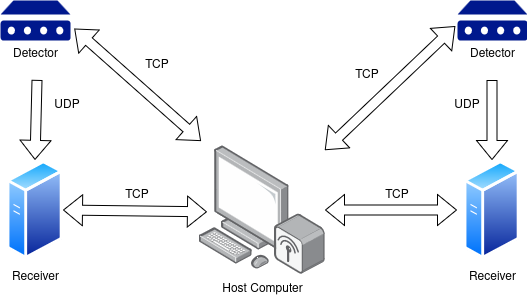
\includegraphics[scale=0.8]{Chapitre1/figures/slsreceiver.png}
        \caption{slsDetectorPackage setup for two detectors. Configuration uses TCP while
            data streaming from detector to slsReceiver uses UDP}
        \label{fig:detector}
    \end{figure}

    \section{Problem Statement}
    \subsection{Existing Solution}
    The detector's group includes scientists, software engineers, firmware engineers, chip designers and many more roles.
    The group is diverse and the libraries' usage differs from one user to another. In general the usage of the libraries includes: acquiring data from network
    , configuring receivers and detectors, storing incoming data, processing data on the fly or after storing it.
    For the standard functionalities users rely on the slsDetectorPackage binaries. But the slsDetectorPackage is a generic software
    developed for public use and has very broad functionalities. Hence, for specific use cases scientists might need to write their own scripts
    or change the slsDetectorPackage source code and build again.
    \subsection{Limits of The Existing Solution}
    The slsDetectorPackage is a very powerful software package, but it has some major limitations.
    \subsubsection{Code Complexity}
    First, the code is very complex and has a steep learning curve. The code is written in C++ and uses
    many advanced features of the language. The code is also very large, with many thousands of lines of code.
    This makes it difficult for new users to understand how the code works, and to modify it to suit their needs.
    In addition, scientists are not software engineers, and in case of a bug, new feature or a specific use case
    they will be exposed to complex code that they are not familiar with. This might include the need to understand
    C++ code, multi-threading, network programming, and many other advanced topics.


    \subsubsection{Code Rigidity}
    Second, the code is very rigid and inflexible. The code is designed to work in a specific way, and it is difficult
    to modify it to work in a different way. This means that scientists are limited in what they can do with the code,
    and they are forced to work within the constraints of the existing code. This can be very frustrating for scientists,
    who may have specific requirements that are not met by the existing code.
    Furthermore, some of the speicific use case code is very brittle and can break easily if the code is modified.
    It lacks proper testing, error handling and logging. This makes it difficult to maintain and extend the code.


    \subsubsection{Code Duplication}
    Third, the code is duplicated in many places. Scientist often rely on their own scripts to perform specific tasks.
    This leads to each scientist having their own version of the code, which is difficult to maintain and update.
    and also results in the use of sub-optimal code, which is not efficient or reliable.


    \subsubsection{Data Storage Limitations}
    As the detectors become more and more advanced, the amount of data that they produce is increasing.
    This has made processing the incoming data in real-time a must. The slsDetectorPackage provides very limited
    functionalities for processing data on the fly. This means that scientists are forced to store the data on disk
    and process it later. This is not ideal and is becoming less practical as the amount of data can be very expensive to
    store and process. The new library should be designed to process around 10GB/s of data in real-time.

    \section{Project Goals}
    The goal of this project is to develop a new library that will address the limitations of the existing software.
    The new software package will be designed to be simple, flexible, and efficient. It will be easy to use, and will be
    designed to meet the needs of scientists and engineers. \\

    The library should include functionalities for acquiring data from receiver servers, stream data to receivers,
    read and write raw data files and numpy files, includes commonly used algorithms for data processing and it should
    expose a C++ and a Python API. \\

    In addition, code should be well tested, documented, and should include logging and error handling.
    The library should be designed to be extensible, so that new features can be added easily in the future.
    and also flexible so that it accomodates different and upcoming use cases. \\

    The library should be designed to be efficient, so that it can process data in real-time, and should be able to handle
    large amounts of data. It should use parallelism to distribute the load on multiple cores, and should be able to
    take advantage of the GPU for processing data. On the other hand it should abstract the low level details of the
    hardware and network communication to make it easy to use for the scientists.




    \section{Work Methodology}
    We used the \textbf{Kanban} methodology to manage the project. Kanban is a subsystem of the Toyota Production System (TPS),
    which was created in 1940s to control inventory levels, the production and
    supply of components, and in some cases, raw material. \cite{junior2010variations}

    The board is divided into several columns:
    \begin{itemize}
        \item \textbf{Backlog} Contains all the tasks that need to be done.
        \item \textbf{To Do} Contains the tasks that are ready to be worked on.
        \item \textbf{In Progress} Contains the tasks that are currently being worked on.
        \item \textbf{Done} Contains the tasks that are completed.
    \end{itemize}

    \subsection{Tools}
    We used Github Projects to manage the Kanban board. Github Projects is a tool that allows you to create a Kanban board
    and manage your tasks. It is integrated with Github, so you can link your tasks to your code, and track your progress
    easily. We also used Github Issues to create tasks, and Github Pull Requests to review and merge the code.

    The Kanban boards were available for all the group members (involved in project or not), so that they can see the progress
    of the project, and contribute to it if needed. The boards were updated regularly, and the progress was tracked using the
    boards. The boards were also used to plan the work, and to assign tasks to the group members.

    \subsection{Benefits of Kanban}
    The Kanban methodology has several benefits:
    \begin{itemize}
        \item \textbf{Visibility} The Kanban board provides a visual representation of the work
              that needs to be done, and the progress that has been made.
        \item \textbf{Flexibility} The Kanban board is flexible, and can be easily adapted to
              the needs of the project.
        \item \textbf{Efficiency} The Kanban board helps to prioritize the work, and to focus
              on the most important tasks.
        \item \textbf{Collaboration} The Kanban board is a collaborative tool, and can
              be used by all the group members to track the progress of the project.

    \end{itemize}

    \subsection{Meetings}
    We had regular meetings with the group members to discuss the progress of the project, and to plan the work.
    On each Tuesday, The whole group meets for about an hour to discuss the progress of the multiple projects that are being worked on.
    This meeting helps to keep everyone informed about the progress of the projects, and to identify any issues that need to be addressed.

    In addition, on each Friday, a one-on-one meeting is held with the project supervisor to discuss the progress made during the week,
    and to plan the work for the next week. This is a more detailed meeting where we discuss the tasks that need to be done, and the
    kep track of the progress of the project.

    Furthermore, the group has an open door policy, where anyone can ask for help, or discuss any issues that they are facing.
    Knowledge sharing is encouraged, and regular short discussions help overcoming the roadblocks that one might encounter.
    \section{High Level Planning}
    Even though the work methodology is highly flexible, we have a high level planning that we follow.
    The project is divided into several phases:
    \begin{itemize}
        \item \textbf{Phase 1: Research and Project Setup} In this phase, we researched the existing solutions, identified the limitations of the existing software,
              setup the project, and developed a high level architecture for the new library.
        \item \textbf{Phase 2: Implementation of the File Module} In this phase, we implemented the file IO module, which is responsible for reading and writing raw data files and numpy files.
        \item \textbf{Phase 3: Implementation of the Network Module} In this phase, we implemented the network module, which is responsible for acquiring data from receiver servers, and streaming data.
        \item \textbf{Phase 4: Implementation of the Processing Module} In this phase, we implemented the processing module, which includes commonly used algorithms for data processing.
        \item \textbf{Phase 5: Implementation of the Python API} In this phase, we implemented the Python API, which allows users to use the library from Python.
        \item \textbf{Phase 6: Documentation, Testing and Evaluation} In this phase, we tested the library more thoroughly, evaluated the performance, documented the code and added tutorials.
    \end{itemize}

    It is important to note that the phases are not fixed, and can be adapted to the needs of the project. The phases are used to plan the work, and to track the progress of the project.
    For example the python API was implemented in parallel with the other modules, as it was very useful to test the library and to get feedback from the users.

    \begin{figure}[h]\centering
        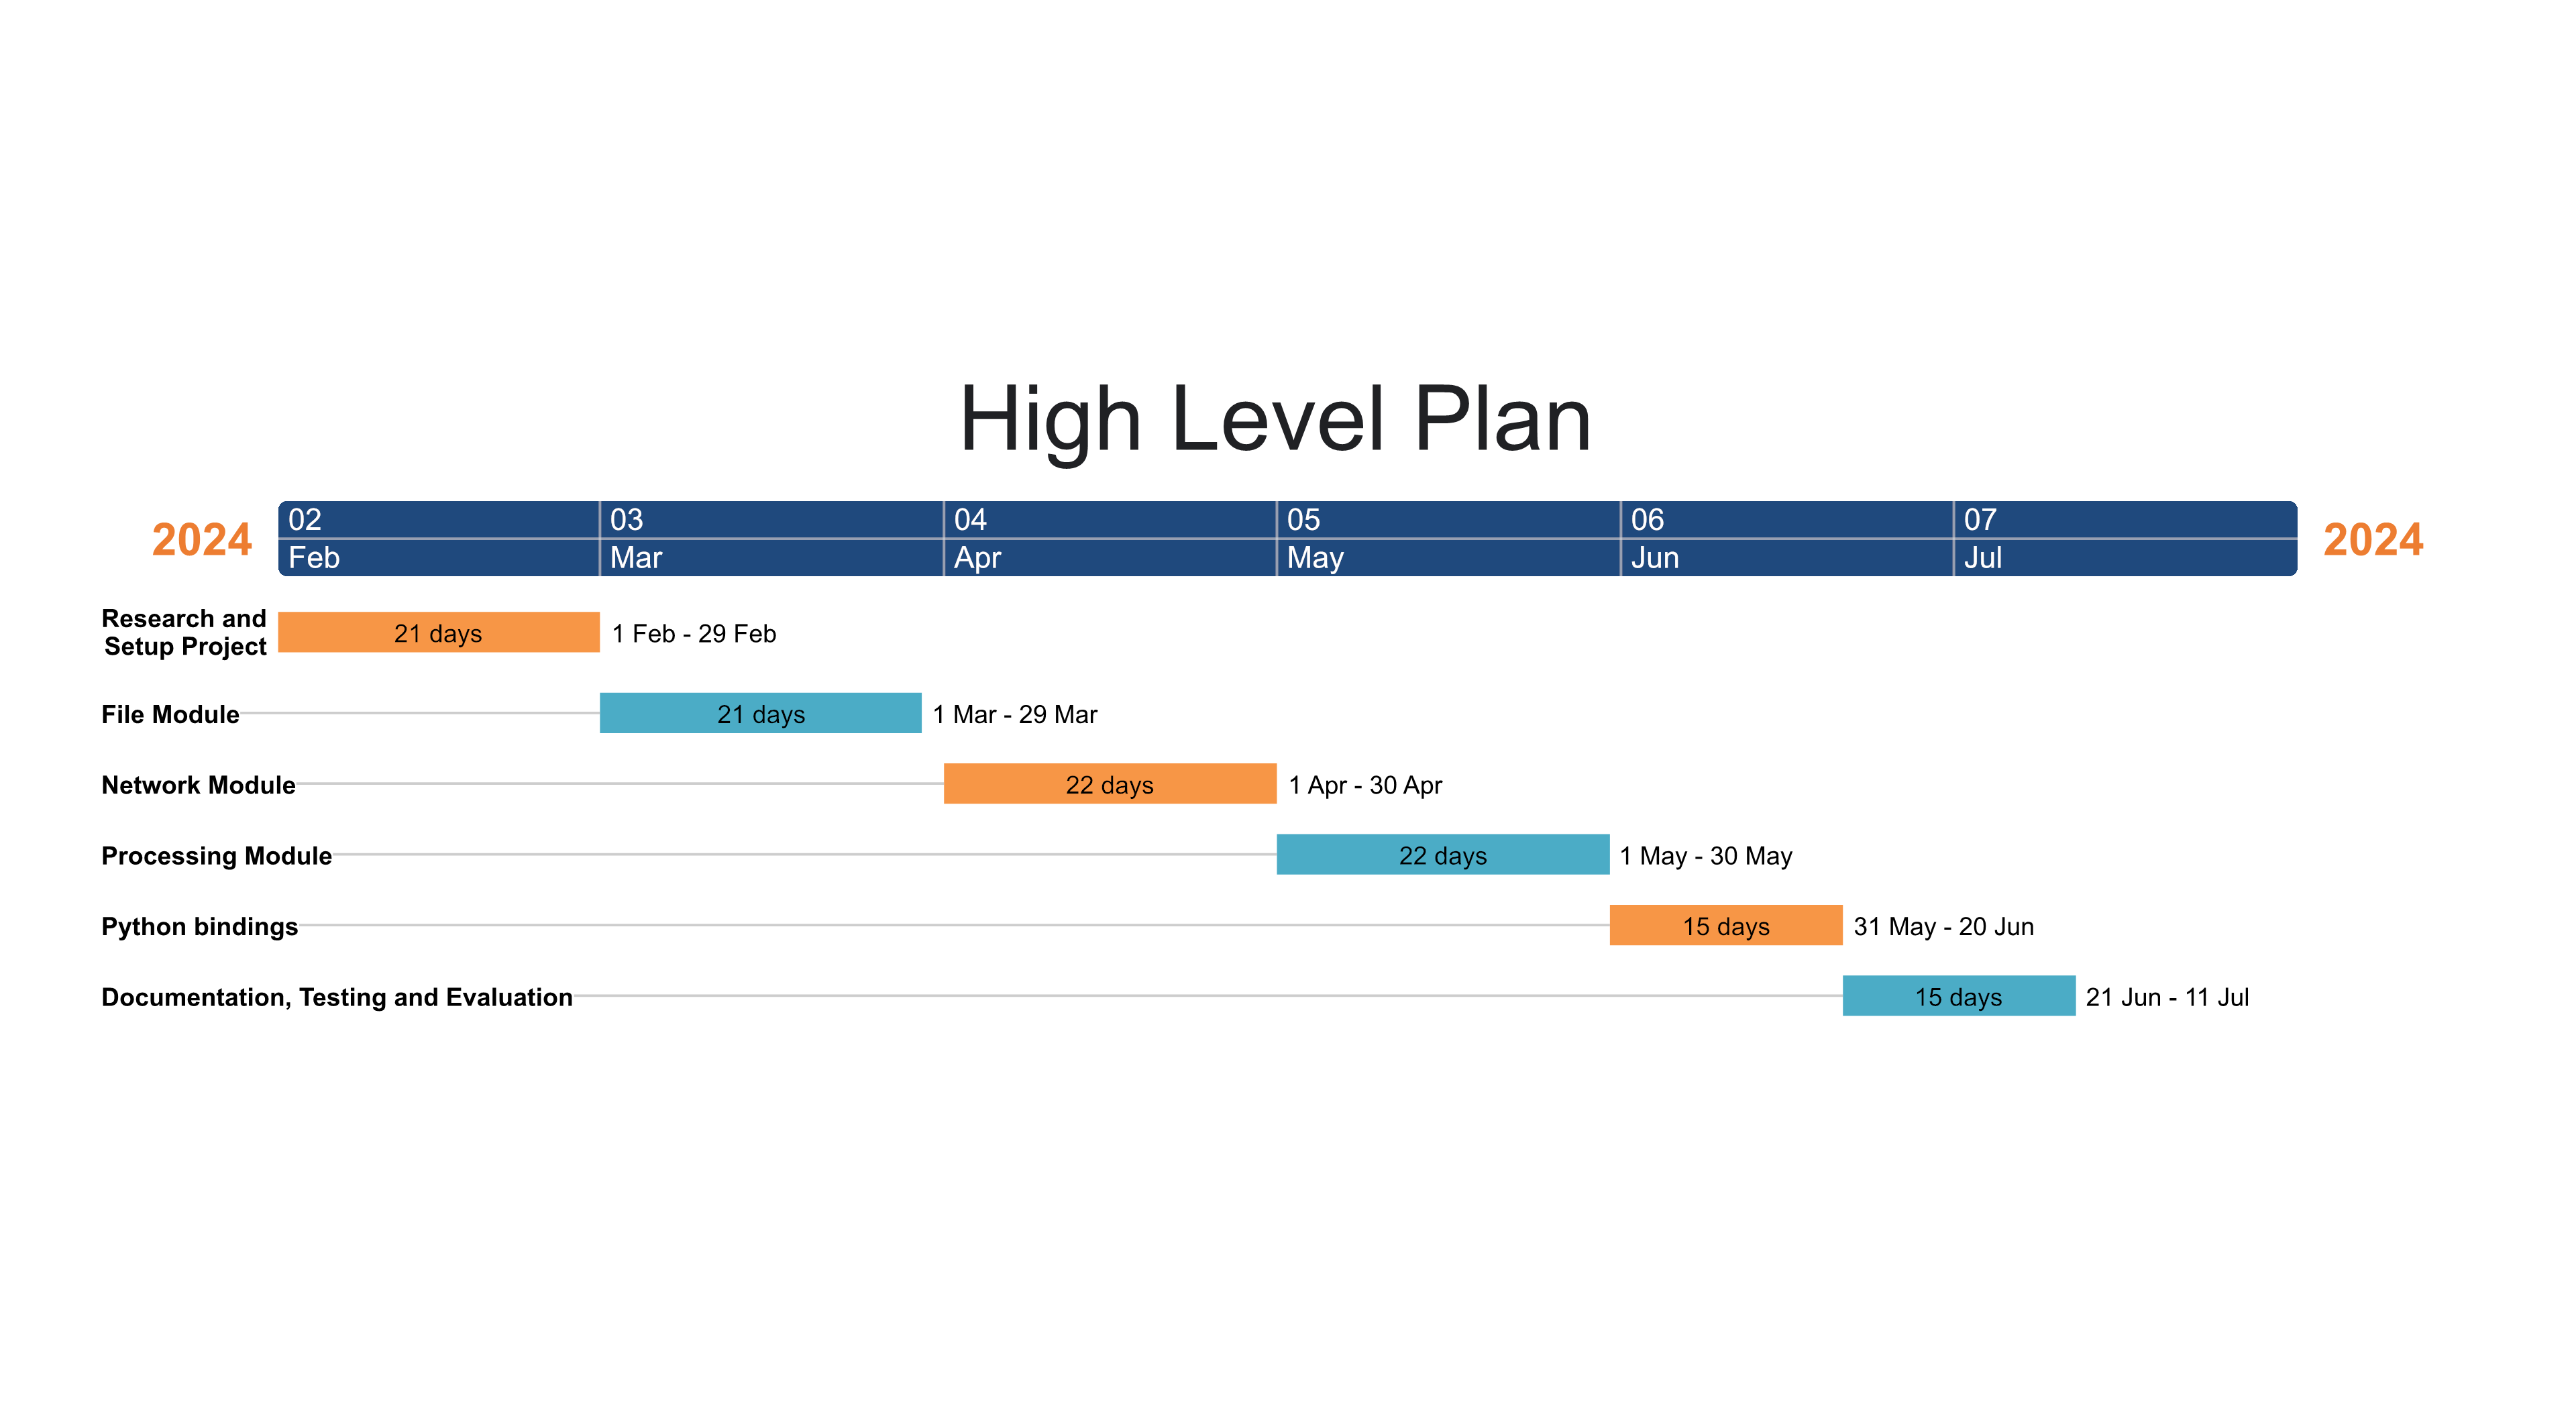
\includegraphics[width=\textwidth]{Chapitre1/figures/gantt.png}
        \caption{Gantt Diagram of the 6 phases of development. A margin was left at the end of the project to account for 
        holidays, vacation days and development delays}
        \label{fig:gantt}
    \end{figure}

    \section*{Conclusion}
    La conclusion est en général sans numérotation, et n'apparaît pas dans la table des matières.


    %==============================================================================
\end{spacing}
